\documentclass[10 pt, a4paper]{article}

\usepackage{graphicx}
\usepackage{caption}
\usepackage{anysize}
%\usepackage{changepage}
\usepackage{amsfonts}
\usepackage{float}
\usepackage{todonotes}
\usepackage{amsmath}
\usepackage[toc,page]{appendix}
\usepackage{subcaption}
\usepackage{hyperref}

\marginsize{2 cm}{2 cm}{1 cm}{2 cm}

\captionsetup[figure]{labelfont=bf,textfont=it,width=0.88\textwidth}
\captionsetup[table]{labelfont=bf,textfont=it,width=0.88\textwidth}

\setlength{\parindent}{0 cm}

\begin{document}


\begin{center}
\huge Studying the Phase Transition in the 2D Square Lattice Zero Field Ising Model using a Convolutional Neural Network \\

\end{center}

\setcounter{figure}{0}

\abstract{The 2D Ising model has a phase transition at a finite temperature $T_C$. The conventional way to study this phase transition is using Markov Chain Monte Carlo (MCMC) to simulate the model at a range of temperatures. In this report we try to use a Convolutional Neural Network to determine the critical temperature by classifying configurations at labelled temperatures generated by MCMC. From the weights of this classification we determined the critical temperature at $k_B T_C / J = 2.23(5)$ which agrees with the analytical results of $k_B T_C / J = \frac{2}{\ln(1 + \sqrt{2})} \simeq 2.2691 \dots$ \cite{onsager}.}


\section{Introduction}

In theoretical physics we study simplified models of nature. One of the widely used models in theoretical physics is the Ising model. This model has a phase transition at a finite value of the order parameter. The conventional way to study this phase transition is by simulating the Ising model using Monte Carlo algorithms to evolve the system from the initial values at a given temperature. It might be insightful to reverse this process (ie. determining the temperature given a final state of the system like a kind of thermometer). The Monte Carlo algorithms commonly used to study the Ising model are irreversible so those can not easily be used to study the reverse of the simulation.

\section{Theoretical Background}

The 2D Ising model consist of spins arranged on a regular 2D lattice. These spins can have a value of $-1$ or $1$. These spins could represent the spin of atoms in a metal. The energy of this system is given by the Hamiltonian 

\begin{align}
H = -J  \sum_{\langle i,j \rangle} \sigma_i \sigma_j -  \mu h \sum_i \sigma_i
\end{align}          

where $J$ is the coupling constant between spins, $\sigma_i$ the spin at lattice site $i$, $\mu$ the coupling constant between the spins and the external field and $h$ the magnitude and the direction of the external magnetic field. The sum $\sum_{\langle i,j \rangle}$ goes over all the nearest neighbour pairs. In order to reduce the complexity of the phase transition we look at the Ising model without external field so we set $h = 0$ which results in the Hamiltonian

\begin{align}
H = -J  \sum_{\langle i,j \rangle} \sigma_i \sigma_j 
\end{align} 

The conventional way to computationally study the 2D Ising model is by using Markov Chain Monte Carlo (MCMC) algorithms. The MCMC algorithm commonly used is the Metropolis algorithm which works by choosing a random lattice site, flip that spin and calculate what that does to the total energy of the system. If the energy decreases accept the flip outright and when the energy increases accept it with the chance given by

\begin{align}
P = e^{- \beta \Delta H}
\end{align}

with $\beta = 1/k_B T$ with $k_B$ the Boltzmann constant and $T$ the temperature. $\Delta H$ is the energy change due to this flip. After taking a number of spins the system equilibrates to a final configuration. At low temperatures the chance of flipping a spin become very small so the system goes to either all spins at $-1$ or $1$. When the temperature increases the chance of flipping a spin becomes higher so at high temperatures the final configuration is a random configuration with magnetisation\footnote{The magnetisation is defined as the total sum over all spins} going to zero. At a finite temperature the system crosses over from the low to the high temperature limit. The temperature at which this phase transition occurs is called the critical temperature $T_C$. Analytically the critical temperature is found to be $k_B T_C / J = \frac{2}{\ln(1 + \sqrt{2})} \simeq 2.2691 \dots $\footnote{The derivation of the analytical critical temperature is beyond the scope of this report, see for example Onsager 1944 \cite{onsager}.}.

\begin{figure}[H] 
\begin{subfigure}[b]{0.33\textwidth}
\begin{figure}[H]
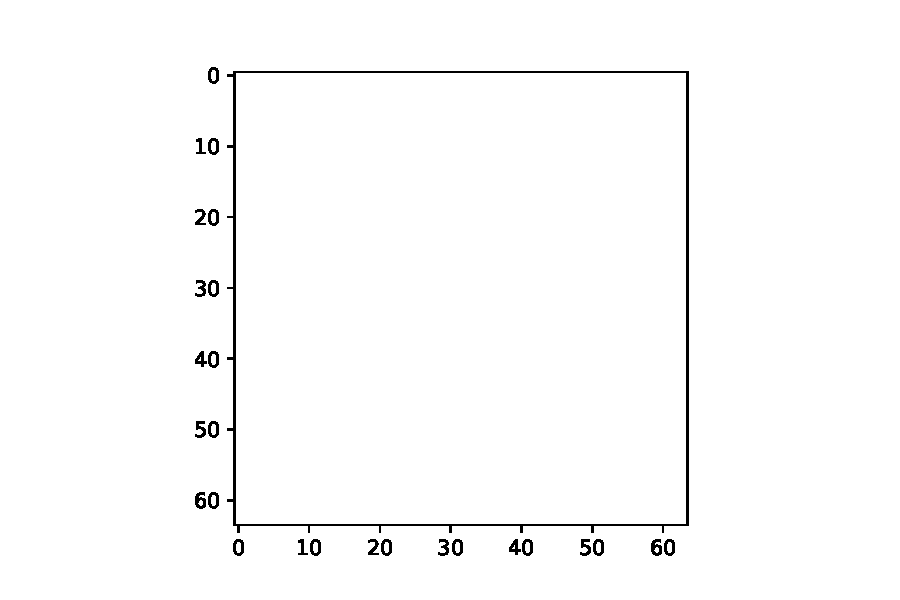
\includegraphics[width=\textwidth]{lattice1}
\caption{$k_B T_C / J = 0.45$.}
\end{figure}
\end{subfigure}
\begin{subfigure}[b]{0.33\textwidth}
\begin{figure}[H]
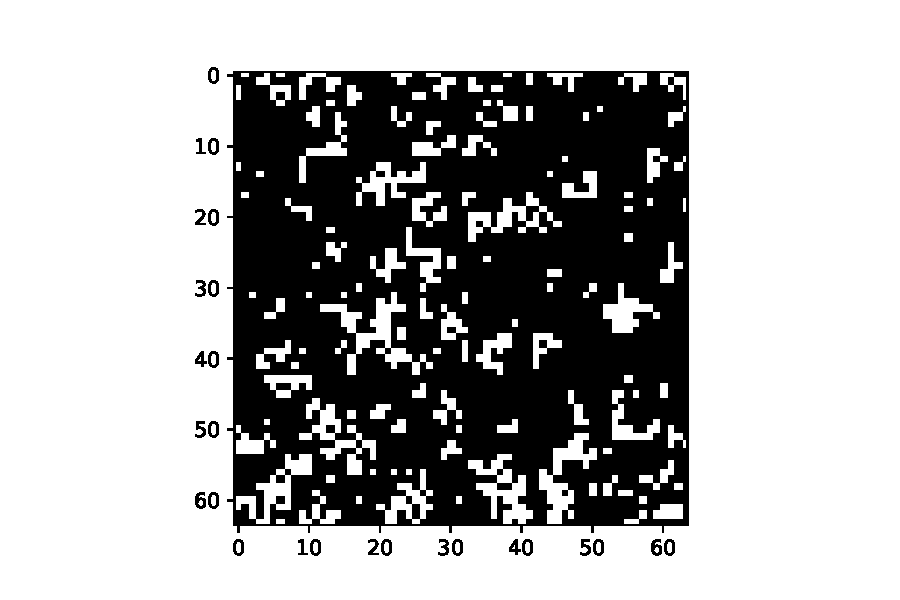
\includegraphics[width=\textwidth]{lattice2}
\caption{$k_B T_C / J = 2.1$.}
\end{figure}
\end{subfigure}
\begin{subfigure}[b]{0.33\textwidth}
\begin{figure}[H] 
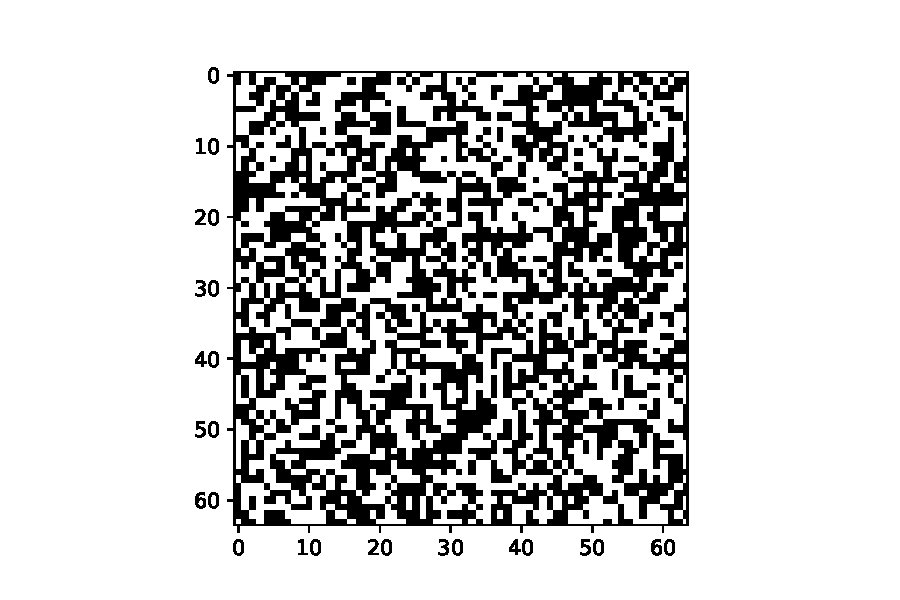
\includegraphics[width=\textwidth]{lattice3}
\caption{$k_B T_C / J = 4.0$.}
\end{figure}
\end{subfigure}
\caption{2D Ising configurations at three temperatures below, around and above the critical temperature respectively. System size of $64 \times 64$ spins. Below the critical temperature all the spins are aligned, above the critical temperature the spins are random which results in zero net spin. }
\label{fig:lattices}
\end{figure}

This process is not reversible so it is not a method to study the reverse process, that is, to determine the critical temperature given a labelled\footnote{The labels are the temperatures at which these configurations are generated.} set of final configuration.
\\
\\
One of the methods to study the 2D Ising model analytically is by using Renormalization Group (RG) methods. RG methods look at how the model changes when we look at the model at different length scales.

\begin{figure}[H] 
\centering
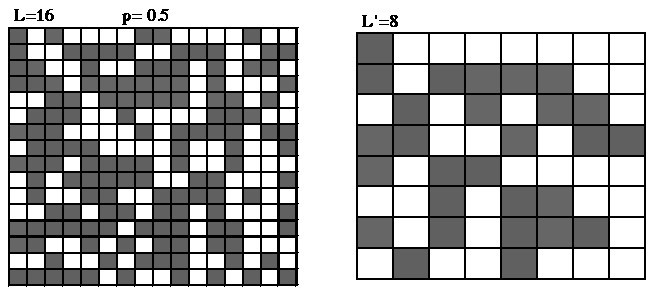
\includegraphics[width=0.7\textwidth]{RG}
\caption{Example of a transformation used in Renormalization Group theory applied to the 2d square lattice Ising model. The technical details not relevant. The RG transformation resembles the effect a convolutional filter has on an image. Source: \cite{RG} }
\label{fig:RG}
\end{figure}

There are parallels between RG methods and the convolutional filters used in convolutional neural networks (CNN). Therefore it might be possible to get insights in the phase transition by applying a CNN to the labelled set. 
\\
\\
In order to make to notation more clear we define a reduced temperature defined by $\hat{T} = k_B T_C / J$ and will from now on drop the hat and use $T$ as the reduced temperature. Likewise we use from now on $\beta$ to mean the inverse reduced temperature.

\section{Methods}

In order to train the CNN we first need to generate the dataset. In order to generate this dataset a program was written that uses the Metropolis algorithm to generate final configurations of lattice size $L$ within a range of temperatures. For the dataset used the parameters were

\begin{table}[H]
\centering
\caption{Parameters used to generate the dataset using MCMC. \label{tab:params}}
\begin{tabular}{l|l}
Parameter: & Value:                                           \\ \hline
$T_\mathrm{min}$ & 0.1                       \\
$T_\mathrm{max}$ & 4.5  \\
$\Delta T$        & $1 \times 10^{-3}$ \\                           
$L$        & 100                           \\
\end{tabular}
\end{table} 

This generated 4400 test configurations. In order to verify that this dataset has a phase transition within this temperature range we can plot the sum over all spins for each point in the temperature range (figure \ref{fig:mags}).

\begin{figure}[H] 
\centering
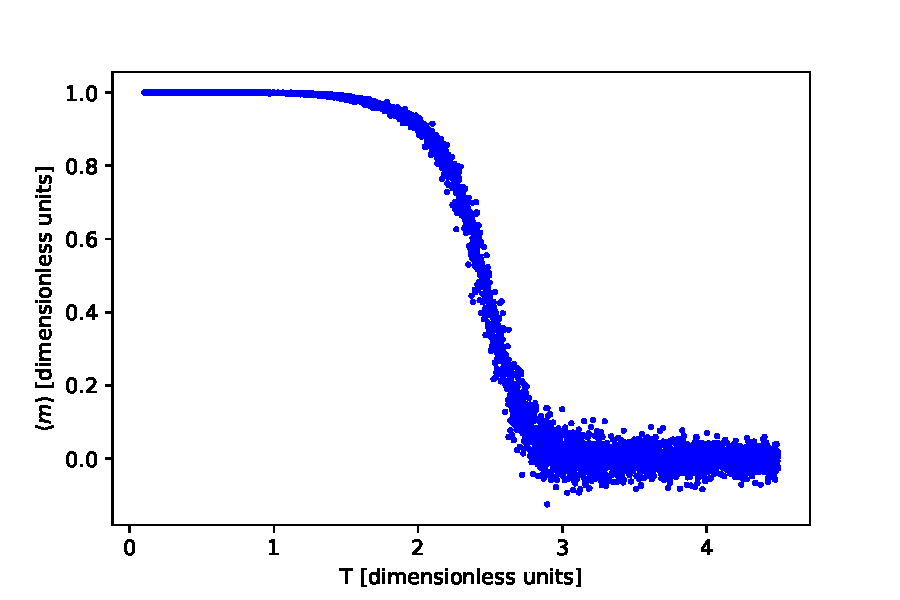
\includegraphics[width=0.7\textwidth]{mag}
\caption{The average magnetisation per spin for the generated data points generated using the parameters as given in table \ref{tab:params}. One can see there is a clear transition happening around the analytical value of $T_C$. \label{fig:mags}}
\end{figure}

We want to train a Neural Network to classify these configurations in temperature classes. Therefore we define a discretized temperature, for convenience we choose to use the inverse temperature $\beta$ to define our classes. The minimal inverse temperature is $\beta_\mathrm{min} = 1/T_\mathrm{max} = 1/4.5 = 0.22$ and we choose our maximum at $\beta_\mathrm{max} = 1$. We discretize this range of inverse temperatures in 100 classes. The final fully connected layer of the network uses these classes.
\\
\\
Before feeding our data to the fully connected layer we apply a Convolutional layer with the parameters given in table \ref{tab:CNNparam}. Before feeding the data from the convolutional layer to the fully connected layer we use a dropout layer of $0.5$ to reduce over fitting.

\begin{table}[H]
\centering
\caption{Parameters used for the Convolutional layer. \label{tab:CNNparam}}
\begin{tabular}{l|l}
Parameter: & Value:                                           \\ \hline
Kernel size & 25                     \\
Stride & 13  \\
Activation function        & Rectified Linear Unit (ReLU) \\                           
\# channels        & 3                           \\
\end{tabular}
\end{table} 


When we apply this network to the generated dataset by updating the weights once each epoch we find that it correctly classifies 25\% of the data points after 300 epochs. When we study the weight matrix of the last layer (see figure \ref{fig:weights}) we can see a transition in the weight matrix between two phases. 

\begin{figure}[H] 
\centering
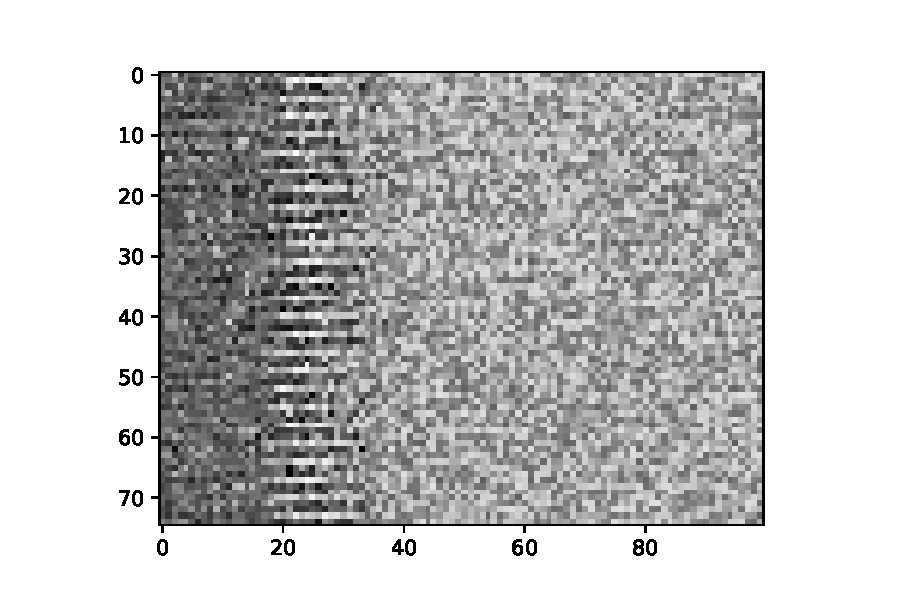
\includegraphics[width=0.7\textwidth]{weights}
\caption{The weight matrix for the final fully connected layer after 300 epochs. The x axis corresponds with the final classes. Around the 25th class there is a phase transistion from dark to random noise. This 25th class coresponds to $\beta = \pm 0.45$ \label{fig:weights}}
\end{figure}

In order to verify whether the temperature of this phase transition agrees with the analytical result we need to quantify the transition position. To do this we sum the weights for each class. So when we look at figure \ref{fig:weights} we sum over each value on the y axis for each class on the x axis. This applied to the weights in figure \ref{fig:weights} is plotted in figure \ref{fig:fit}. In order to find a value for $T_C$ we need to find where the transition occurs. In order to do that we fit a function to the points. Inspired by Tanaka \& Tomiya (2017) \cite{phasemethod} we fit to

\begin{align*}
W(\beta) = a \tanh(c(x - \beta_C)) - b
\end{align*}

and find $\beta_C = 0.449(9)$ which gives a critical temperature of $T_C = 2.23(5)$ which agrees with the analytical value of $T_C = 2.2691 \dots$. The neural network which managed to correctly find the critical temperature only managed to correctly classify the temperature with an accuracy of 25\%.

\begin{figure}[H] 
\centering
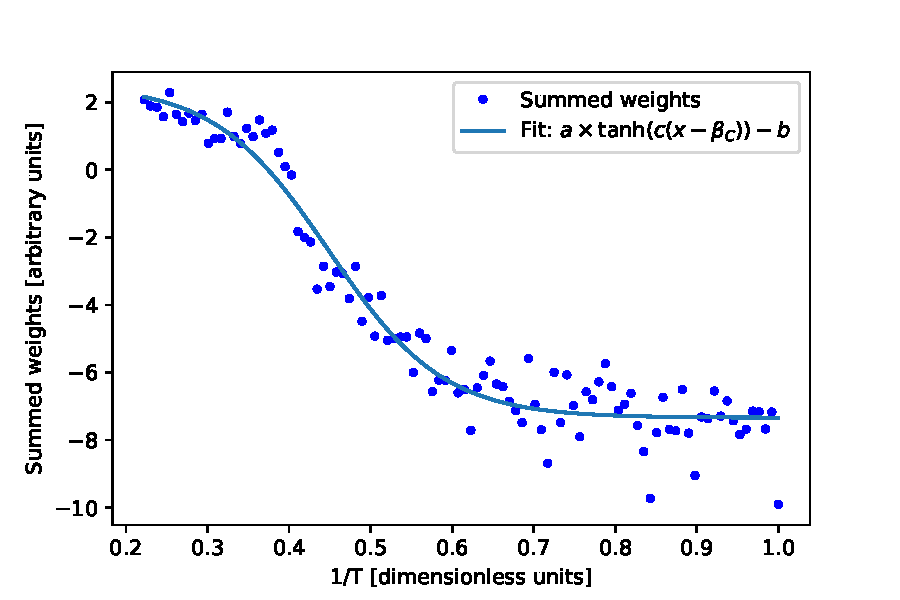
\includegraphics[width=0.7\textwidth]{fit}
\caption{The sums of the weights after 300 epochs for each class of the inverse temperature for the weights in figure \ref{fig:weights} with a fitted $\tanh$ function to find the critical inverse temperature at $\beta_C = 0.449(9)$. \label{fig:fit}}
\end{figure}

The model that manages to correctly determine the critical temperature only correctly classifies with an accuracy of 25\%. This accuracy was achieved after 300 epochs. When we train the network for more epochs the accuracy increases but the phase transition in the weight matrix of the last layer becomes less defined and therefore it becomes more difficult to determine the critical temperature. In figure \ref{fig:fitwrong} we can see the summed weights after 1000 epochs were we can see that the phase transition becomes less well defined and the fitted function does not manage to properly fit the data. The accuracy after 1000 epochs does increase to 37\%.

\begin{figure}[H] 
\centering
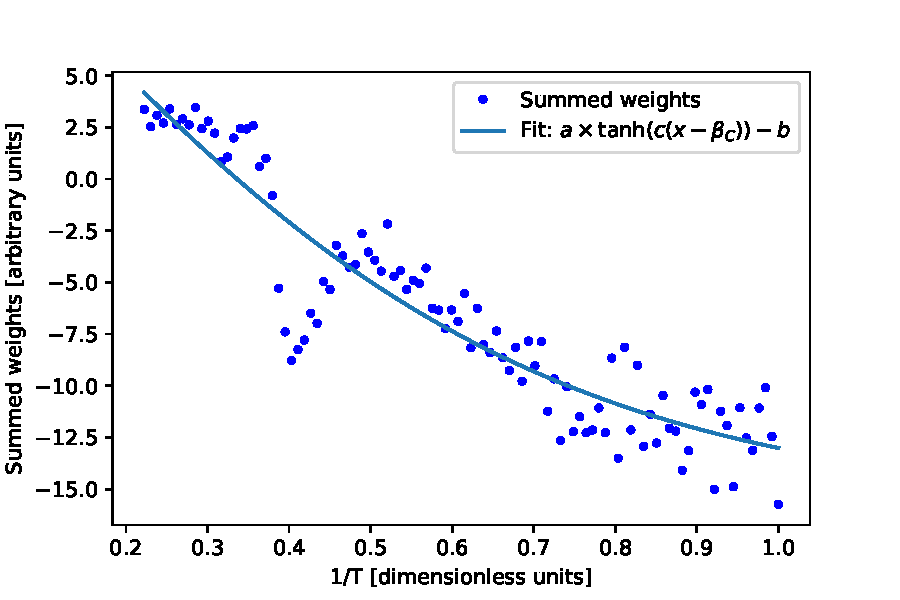
\includegraphics[width=0.7\textwidth]{fitwrong}
\caption{The sums of the weights after 1000 epochs for each class of the inverse temperature for the weights in figure \ref{fig:weightswrong} with a fitted $\tanh$ function where we can see that the fit does not fit the data properly. \label{fig:fitwrong}}
\end{figure}

\begin{figure}[H] 
\centering
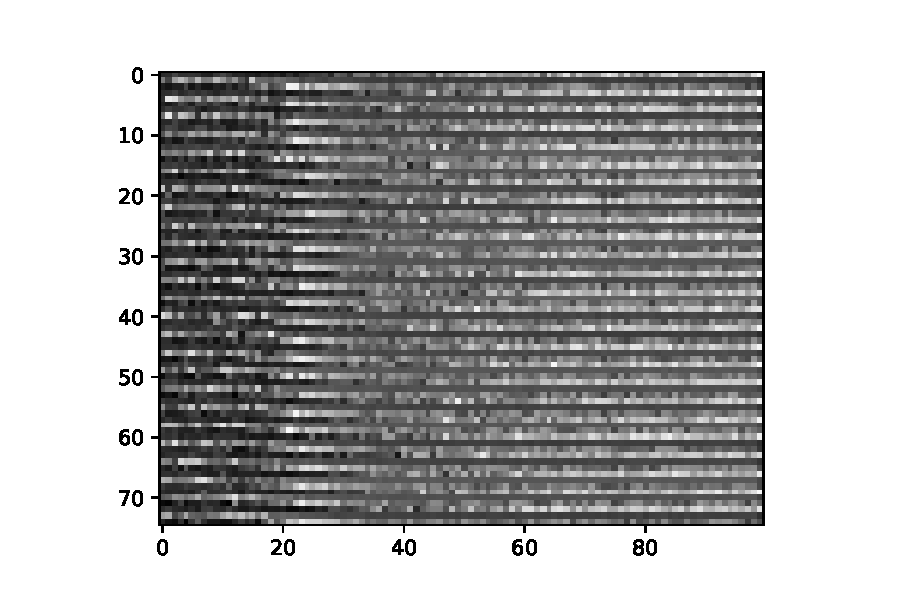
\includegraphics[width=0.7\textwidth]{weightswrong}
\caption{The weight matrix for the final fully connected layer after 1000 epochs. The x axis corresponds with the final classes. The transistion that was visible in figure \ref{fig:weights} after 300 epochs has become less clear.  \label{fig:weightswrong}}
\end{figure}

When we calculate the estimate for the inverse critical temperature every 10 epochs (figure \ref{fig:epochs}) we see that it slowly increases towards the analytical value (indicated by the black line) until after about 500 epochs the phase transition becomes less clear and the estimate for the inverse critical temperature goes to zero. This might be due to over fitting, this might be reduced by adding extra convolutional layers to the model.

\begin{figure}[H] 
\centering
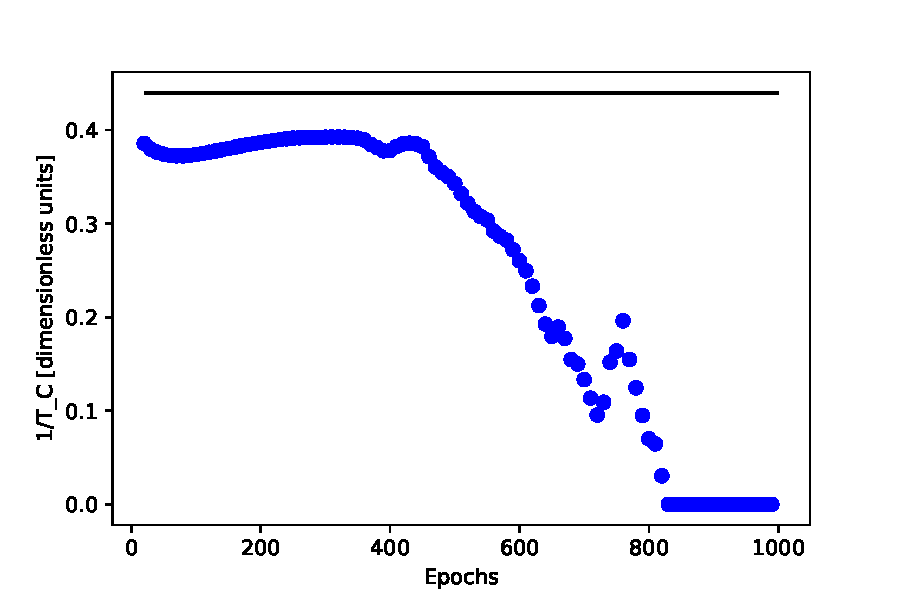
\includegraphics[width=0.7\textwidth]{epochs}
\caption{The estimate for the critical inverse temperature vs. the number of epochs. After around 500 epochs the phase transistion in the weights becomes less clear and therefore the estimate of the critical temperature deviates further from the analytical result represented by the black line. \label{fig:epochs}}
\end{figure}

\section{Conclusion}

We used a simple CNN to find the critical temperature of the zero field Ising model to be $T_C = 2.23(5)$ which agrees with the analytical result of $T_C = \frac{2}{\ln(1 + \sqrt{2})} \simeq 2.2691 \dots$. The only information needed to find this critical temperature was the temperature of equilibrium configurations at a range of temperatures. This method therefore is able to find the critical temperature of a theoretical model without information regarding the phase transition.
\\
\\
For the zero field Ising model a very simple network consisting of only one convolutional layer and one fully connected layer was able to perform this correct determination of the critical temperature. An extension could be to repeat this analysis for the non zero field Ising model and construct the phase diagram for this model.
\\
\\
Using more complex networks it might be possible to extend this method to more complex models like the Potts model or to models of active systems like the Vicsek model.

\begin{thebibliography}{99}

\bibitem{onsager}
L. Onsager (1944), \textit{"Crystal statistics. I. A two-dimensional model with an order-disorder transition"}, Physical Review, Series II, 65 (3–4): 117–149.

\bibitem{RG}
D. Johnson, Phase Transitions, Finite-size Scaling and Renormalization Group, \url{http://schleife.web.engr.illinois.edu/teaching/mse485/lnotes/scaling.html}, retrieved on 2019-04-18.

\bibitem{phasemethod}
A. Tanaka \& A. Tomiya (2017), \textit{Detection of Phase Transition via Convolutional Neural Networks}, Journal of the Physical Society of Japan 86, 063001.
\end{thebibliography}

\end{document}